\documentclass[../../main.tex]{subfiles}
\graphicspath{{../../image/}{../../figure/}}
\begin{document}

\section{解的界}\label{section:ch12-解的界}

我们考虑如上归一化的解，它满足
\begin{align}
|z(x,t)|+|w(x,t)|<2\delta,\qquad -\infty<x<\infty,\ 0<t<\infty,
\label{align:ch12-解小振荡}
\end{align}
其中 $\delta$ 是小正常数。方便起见，将初始数据视为多值函数，允许 $(z(x,0),w(x,0))$ 取以 $(z(x\pm,0),w(x\pm,0))$ 为左右状态的 Riemann 问题解值域中的任一状态。上确界与总变差按使这些量最大的选取来度量。我们进而假设
\begin{align}
\sup_{(-\infty,\infty)}|z(\cdot,0)|+\sup_{(-\infty,\infty)}|w(\cdot,0)|\leqslant\delta,
\label{align:ch12-初值上确界}\\
TV_{(-\infty,\infty)}z(\cdot,0)+TV_{(-\infty,\infty)}w(\cdot,0)<a\delta^{-1},
\label{align:ch12-初值总变差}
\end{align}
其中 $a$ 是小常数，将在稍后独立于 $\delta$ 取定。于是存在一种权衡：允许总变差任意大，代价是保持振荡充分小。目标是建立解的界。在下文，$c$ 表示仅依赖于 $F$ 的一般常数。主要结果是

\begin{theorem}\label{theorem:ch12-TV界}
考虑上半平面中任一类空曲线 $t=t^*(x)$，$x_\ell\leqslant x\leqslant x_r$，沿其 $(z,w)$ 的迹记为 $(z^*,w^*)$。则
\begin{align}
TV_{[x_\ell,x_r]}z^*(\cdot)&\leqslant TV_{[\xi_\ell(0),\xi_r(0)]}z(\cdot,0)+c\delta^2\{TV_{[\zeta_\ell(0),\zeta_r(0)]}z(\cdot,0)+TV_{[\zeta_\ell(0),\zeta_r(0)]}w(\cdot,0)\},
\label{align:ch12-TV界z}\\
TV_{[x_\ell,x_r]}w^*(\cdot)&\leqslant TV_{[\zeta_\ell(0),\zeta_r(0)]}w(\cdot,0)+c\delta^2\{TV_{[\zeta_\ell(0),\xi_r(0)]}z(\cdot,0)+TV_{[\zeta_\ell(0),\xi_r(0)]}w(\cdot,0)\},
\label{align:ch12-TV界w}
\end{align}
其中 $\xi_\ell(\cdot)$、$\xi_r(\cdot)$ 是从图 $t^*(\cdot)$ 的端点 $(x_\ell,t_\ell)$、$(x_r,t_r)$ 发出的极小后向 1-特征线，$\zeta_\ell(\cdot)$、$\zeta_r(\cdot)$ 是极大后向 2-特征线。
\end{theorem}

由于广义特征线是类空曲线，可将上述命题与\cref{theorem:ch12-传播主定理}及假设\eqref{align:ch12-解小振荡}、\eqref{align:ch12-初值总变差}结合，推出下述推论：

\begin{theorem}\label{theorem:ch12-逐点界}
对上半平面任一点 $(x,t)$：
\begin{align}
\sup_{(-\infty,\infty)}z(\cdot,0)\geqslant z(x,t)\geqslant\inf_{(-\infty,\infty)}z(\cdot,0)-ca\delta,
\label{align:ch12-逐点界z}\\
\sup_{(-\infty,\infty)}w(\cdot,0)\geqslant w(x,t)\geqslant\inf_{(-\infty,\infty)}w(\cdot,0)-ca\delta.
\label{align:ch12-逐点界w}
\end{align}
\end{theorem}

于是，由假设\eqref{align:ch12-初值上确界}并选取 $a$ 充分小，我们后验地确保解满足\eqref{align:ch12-解小振荡}。

证明\cref{theorem:ch12-TV界}的工作相当繁重，需要大量准备。在证明过程中，我们将验证度量波相互作用总量的某些量也是有界的。

考虑一个 1-激波，连接左状态 $(z_-,w_-)$ 与右状态 $(z_+,w_+)$。跳跃量 $\Delta z=z_+-z_-$ 与 $\Delta w=w_+-w_-$ 通过方程
\begin{align}
\Delta w=f(\Delta z;z_-,w_-)
\label{align:ch12-1激波参数}
\end{align}
相联系，该方程由从状态 $(z_-,w_-)$ 发出的 1-激波曲线的重新参数化产生。特别地，$f$ 及其关于 $\Delta z$ 的前两阶导数在 $\Delta z=0$ 处为零，故当 $\Delta z\to0$ 时，$f$、$\partial f/\partial z_-$ 与 $\partial f/\partial w_-$ 均为 $O(\Delta z^3)$。

类似地，连接左状态 $(z_-,w_-)$ 与右状态 $(z_+,w_+)$ 的 2-激波两侧 Riemann 不变量的跳跃量 $\Delta w=w_+-w_-$ 与 $\Delta z=z_+-z_-$ 通过方程
\begin{align}
\Delta z=g(\Delta w;z_+,w_+)
\label{align:ch12-2激波参数}
\end{align}
相联系，该方程由从状态 $(z_+,w_+)$ 发出的后向 2-激波曲线（原书第 9.3 节）的重新参数化产生。
进而，当 $\Delta w\to0$ 时，$g$ 连同 $\partial g/\partial z_+$ 与 $\partial g/\partial w_+$ 均为 $O(\Delta w^3)$。

为方便起见，上半平面的点用单个大写字母 $I$、$J$ 等标记。对任一点 $I=(\bar x,\bar t)$，我们按\cref{section:ch12-解的局部结构}所述并如\cref{figure:ch12-八曲线}所示，与之相联系特殊特征线 $\varphi_\pm^I$、$\psi_\pm^I$、$\xi_\pm^I$、$\zeta_\pm^I$，并识别当 $I$ 从扇形 $\mathscr{S}_W^I$、$\mathscr{S}_E^I$、$\mathscr{S}_N^I$、$\mathscr{S}_S^I$ 趋近时的极限 $(z_W^I,w_W^I)$、$(z_E^I,w_E^I)$、$(z_N^I,w_N^I)$、$(z_S^I,w_S^I)$。从 $I$ 发出极小 1-分隔线 $p_\pm^I$ 与极大 2-分隔线 $q_\pm^I$，其构造如下：$p_-^I$（或 $q_+^I$）即从 $I$ 发出的极小（或极大）后向 1-特征线 $\xi_-^I$（或 2-特征线 $\zeta_+^I$）；而 $p_+^I$（或 $q_-^I$）是从 $\mathscr{S}_E^I$（或 $\mathscr{S}_W^I$）中点 $(x_n,t_n)\to(\bar x,\bar t)$（$n\to\infty$）发出的极小（或极大）后向 1-特征线 $\xi_n$（或 2-特征线 $\zeta_n$）序列的极限。引入记号
\begin{align}
\mathscr{F}_I&=\{(x,t):0\leqslant t<\bar t,\ p_-^I(t)\leqslant x\leqslant p_+^I(t)\},
\label{align:ch12-FI}\\
\mathscr{G}_I&=\{(x,t):0\leqslant t<\bar t,\ q_-^I(t)\leqslant x\leqslant q_+^I(t)\}.
\label{align:ch12-GI}
\end{align}
由\cref{theorem:ch12-局部正则存在}与\cref{theorem:ch12-传播主定理}，
\begin{align}
\lim_{t\uparrow\bar t}z(p_-^I(t),t)=z_S^I,\qquad \lim_{t\uparrow\bar t}z(p_+^I(t),t)=z_E^I,
\label{align:ch12-p极限z}\\
\lim_{t\uparrow\bar t}w(q_-^I(t),t)=w_W^I,\qquad \lim_{t\uparrow\bar t}w(q_+^I(t),t)=w_S^I.
\label{align:ch12-q极限w}
\end{align}

在 $I$ 处入射的 1-波与 2-波的累积强度分别度量为
\begin{align}
\Delta z^I=z_E^I-z_S^I,\qquad \Delta w^I=w_S^I-w_W^I.
\label{align:ch12-入射波}
\end{align}
若仅允许入射 1-波相互作用，它们将产生一个 $w$-振幅为
\begin{align}
\Delta w_*^I=f(\Delta z^I;z_S^I,w_S^I),
\label{align:ch12-出波w}
\end{align}
的出射 1-激波以及一个出射 2-稀疏波。因此，$|\Delta w_*^I|$ 超过入射 1-波的累积 $w$-强度 $|w_E^I-w_S^I|$。类似地，仅入射 2-波的相互作用将产生一个 $z$-振幅为
\begin{align}
\Delta z_*^I=g(\Delta w^I;z_S^I,w_S^I),
\label{align:ch12-出波z}
\end{align}
的出射 2-激波，超过其累积 $z$-强度 $z_S^I-z_W^I$。注意，若 $z_S^I=z_W^I$、$w_S^I=w_W^I$，则 $\Delta w_*^I=w_N^I-w_W^I$；而若 $z_S^I=z_E^I$、$w_S^I=w_E^I$，则 $\Delta z_*^I=z_E^I-z_N^I$。

我们将上半平面可视作一个偏序集，其偏序关系由规则 $I<J$ 诱导：每当 $J$ 被限制在从 $I$ 发出的极小 1-分隔线 $p_-^I$ 与 $p_+^I$ 的图像之间。特别地，当 $J$ 严格位于 $p_-^I$ 图像之右时，$I$ 位于从 $J$ 发出的 1-特征线 $\phi_-^J$ 的图像上。于是 $I<J$ 蕴含 $I$ 总位于从 $J$ 发出的某条前向 1-特征线的图像上，即 $\phi_-^J$ 或 $p_-^J$。这一特殊特征线记为 $\chi_-^J$。

我们考虑 1-特征线树 $\mathscr{M}$，它由上半平面的有限点集（称为节点）组成，并具有下述性质：$\mathscr{M}$ 含唯一极小节点 $I_0$，即树的根。进而，若 $J$ 与 $K$ 是任意两个节点，则穿过根 $I_0$ 的前向 1-特征线 $\chi_-^J$ 与 $\chi_-^K$ 的汇合点 $I$ 也是 $\mathscr{M}$ 的节点。一般地，$\mathscr{M}$ 含若干极大节点（\cref{figure:ch12-特征线树}）。

每个节点 $J\neq I_0$ 相对于 $\mathscr{M}$ 连续于某节点 $I$，即它是 $\mathscr{M}$ 中以 $I$ 为严格最大下界的节点。连续于节点 $I$ 的节点集记为 $\mathscr{C}_I$。当 $J$ 连续于 $I$ 时，配对 $(I,J)$ 称为一条链节。节点的有限序列 $\{I_0,I_1,\cdots,I_m\}$，其中 $I_{j+1}$ 连续于 $I_j$（$j=0,\cdots,m-1$），连接根 $I_0$ 与某极大节点 $I_m$，构成 $\mathscr{M}$ 的一条链。

若 $(I,J)$ 是 $\mathscr{M}$ 的一条链节，即 $I=(\chi_-^J(\bar t),\bar t)$，令
\begin{align}
z_\pm^{IJ}=\lim_{t\uparrow\bar t}z(\chi_-^J(t)\pm,t),\qquad
w_\pm^{IJ}=\lim_{t\uparrow\bar t}w(\chi_-^J(t)\pm,t),
\label{align:ch12-链节极限}
\end{align}
\begin{align}
\Delta z^{IJ}=z_+^{IJ}-z_-^{IJ},\qquad
\Delta w^{IJ}=w_+^{IJ}-w_-^{IJ}.
\label{align:ch12-链节跳跃}
\end{align}
特别地，
\begin{align}
\Delta w^{IJ}=f(\Delta z^{IJ};z_-^{IJ},w_-^{IJ}).
\label{align:ch12-链节f}
\end{align}

\begin{figure}[ht]
\centering
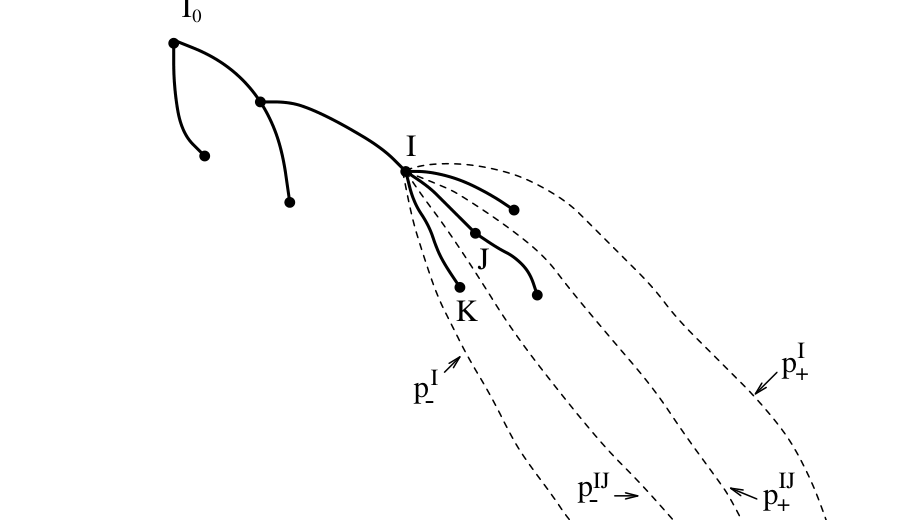
\includegraphics[width=0.75\textwidth]{ch12-fig05-01.png}
\caption{1-特征线树：根 $I_0$、节点 $I,J,K$ 与分隔线 $p_\pm^I,p_\pm^{IJ}$}
\label{figure:ch12-特征线树}
\end{figure}

与链节 $(I,J)$ 相联系，我们构造从 $I$ 发出的极小 1-分隔线 $p_\pm^{IJ}$，其方式如下：$p_-^{IJ}$ 是从点 $(\chi_-^J(t),t)$ 发出的极小后向 1-特征线族 $\xi_t$ 在 $t\uparrow\bar t$ 时的极限；而 $p_+^{IJ}$ 是从满足 $t_n\uparrow\bar t$、$x_n-\chi_-^J(t_n)\downarrow0$、$z(x_n-,t_n)\to z_+^{IJ}$、$w(x_n-,t_n)\to w_+^{IJ}$ 的点 $(x_n,t_n)$ 发出的极小后向 1-特征线序列 $\xi_n$ 的极限。注意，$p_\pm^{IJ}$ 的图像被限制在 $p_-^I$ 与 $p_+^I$ 的图像之间（见\cref{figure:ch12-特征线树}）。进而，对任意 $K>J$，$p_\pm^K$ 的图像被限制在 $p_-^{IJ}$ 与 $p_+^{IJ}$ 的图像之间。此外，
\begin{align}
\lim_{t\uparrow\bar t}z(p_-^{IJ}(t),t)=z_-^{IJ},\qquad
\lim_{t\uparrow\bar t}z(p_+^{IJ}(t),t)=z_+^{IJ}.
\label{align:ch12-pIJ极限}
\end{align}
事实上，上述两式中的第一式已在\cref{lemma:ch12-后向特征极限}证明中（以不同记号；见\eqref{align:ch12-z等式}）建立；第二式可由类似论证验证。

现令
\begin{align}
\mathscr{P}_1(\mathscr{M})&=-\sum_{I\in\mathscr{M}}\left[\Delta w_*^I-\sum_{J\in\mathscr{C}_I}\Delta w^{IJ}\right],
\label{align:ch12-P1}\\
\mathscr{Q}_1(\mathscr{M})&=\sum_{I\in\mathscr{M}}\sum_{J\in\mathscr{C}_I}|\Delta w^{IJ}-\Delta w_*^J|.
\label{align:ch12-Q1}
\end{align}
由\eqref{align:ch12-正则1w}，
\begin{align}
\sum_{J\in\mathscr{C}_I}\Delta w^{IJ}\geqslant w_E^I-w_S^I\geqslant\Delta w_*^I,
\label{align:ch12-和非负}
\end{align}
故 $\mathscr{P}_1$ 与 $\mathscr{Q}_1$ 均非负。

对上半平面的子集 $\mathscr{F}$，我们联系泛函
\begin{align}
\mathscr{P}_1(\mathscr{F})&=\sup_{\mathscr{J}}\sum_{\mathscr{M}\in\mathscr{J}}\mathscr{P}_1(\mathscr{M}),
\label{align:ch12-P1F}\\
\mathscr{Q}_1(\mathscr{F})&=\sup_{\mathscr{J}}\sum_{\mathscr{M}\in\mathscr{J}}\mathscr{Q}_1(\mathscr{M}),
\label{align:ch12-Q1F}
\end{align}
其中 $\mathscr{J}$ 表示含于 $\mathscr{F}$ 的 1-特征线树 $\mathscr{M}$ 的任一（有限）集合，这些树两两不交，意指其中任意两棵的根不可比较。可将 $\mathscr{P}_1(\mathscr{F})$ 视为 $\mathscr{F}$ 内部 1-波相互作用总量的度量，而 $\mathscr{Q}_1(\mathscr{F})$ 为由与 2-波相互作用诱导的 1-激波增强的度量。

我们为 2-特征族引入相应概念：每当 $J$ 被限制在从 $I$ 发出的极大 2-分隔线 $q_-^I$ 与 $q_+^I$ 的图像之间时，规定 $I<J$。在此情形，$I$ 位于从 $J$ 发出的前向 2-特征线 $\chi_+^J$ 的图像上，即 $\psi_+^J$ 或 $q_+^J$。于是可如上构造 2-特征线树 $\mathscr{N}$（含节点、根、链节与链）。在\eqref{align:ch12-链节极限}、\eqref{align:ch12-链节跳跃}与\eqref{align:ch12-链节f}的位置，我们有
\begin{align}
z_\pm^{IJ}&=\lim_{t\uparrow\bar t}z(\chi_+^J(t)\pm,t),\qquad
w_\pm^{IJ}=\lim_{t\uparrow\bar t}w(\chi_+^J(t)\pm,t),
\label{align:ch12-链节极限2}\\
\Delta z^{IJ}&=z_+^{IJ}-z_-^{IJ},\qquad
\Delta w^{IJ}=w_+^{IJ}-w_-^{IJ},
\label{align:ch12-链节跳跃2}\\
\Delta z^{IJ}&=g(\Delta w^{IJ};z_+^{IJ},w_+^{IJ}).
\label{align:ch12-链节g}
\end{align}
与链节 $(I,J)$ 相联系，我们从 $I$ 发出极大 2-分隔线 $q_\pm^{IJ}$，与 $p_\pm^{IJ}$ 类比。$q_\pm^{IJ}$ 的图像被限制在 $q_-^I$ 与 $q_+^I$ 的图像之间；而 $q_\mp^{IJ}$ 的图像被限制在 $q_-^{IJ}$ 与 $q_+^{IJ}$ 的图像之间。在\eqref{align:ch12-pIJ极限}的位置，
\begin{align}
\lim_{t\uparrow\bar t}w(q_-^{IJ}(t),t)=w_-^{IJ},\qquad
\lim_{t\uparrow\bar t}w(q_+^{IJ}(t),t)=w_+^{IJ}.
\label{align:ch12-qIJ极限}
\end{align}
还定义\eqref{align:ch12-P1}与\eqref{align:ch12-Q1}的类比：
\begin{align}
\mathscr{P}_2(\mathscr{N})&=\sum_{I\in\mathscr{N}}\left[\Delta z_*^I-\sum_{J\in\mathscr{C}_I}\Delta z^{IJ}\right],
\label{align:ch12-P2}\\
\mathscr{Q}_2(\mathscr{N})&=\sum_{I\in\mathscr{N}}\sum_{J\in\mathscr{C}_I}|\Delta z^{IJ}-\Delta z_*^J|,
\label{align:ch12-Q2}
\end{align}
它们非负，因为
\begin{align}
\sum_{J\in\mathscr{C}_I}\Delta z^{IJ}\leqslant z_S^I-z_W^I\leqslant\Delta z_*^I.
\label{align:ch12-和非负2}
\end{align}
这诱导出与 $\mathscr{P}_1$、$\mathscr{Q}_1$ 类似的泛函：
\begin{align}
\mathscr{P}_2(\mathscr{F})&=\sup_{\mathscr{J}}\sum_{\mathscr{N}\in\mathscr{J}}\mathscr{P}_2(\mathscr{N}),
\label{align:ch12-P2F}\\
\mathscr{Q}_2(\mathscr{F})&=\sup_{\mathscr{J}}\sum_{\mathscr{N}\in\mathscr{J}}\mathscr{Q}_2(\mathscr{N}).
\label{align:ch12-Q2F}
\end{align}

\begin{lemma}\label{lemma:ch12-不相交求和}
设 $\mathscr{F}_1,\cdots,\mathscr{F}_m$ 是含于上半平面中某集合 $\mathscr{F}$ 的子集族。假设对任意可比较的 $I\in\mathscr{F}_i$ 与 $J\in\mathscr{F}_j$（设 $I<J$），连接 $J$ 到 $I$ 的特征线 $\chi_-^J$（或 $\chi_+^J$）的弧含于 $\mathscr{F}$。则
\begin{align}
\sum_{i=1}^m\{\mathscr{P}_1(\mathscr{F}_i)+\mathscr{Q}_1(\mathscr{F}_i)\}\leqslant k\{\mathscr{P}_1(\mathscr{F})+\mathscr{Q}_1(\mathscr{F})\},
\label{align:ch12-不相交1}
\end{align}
或
\begin{align}
\sum_{i=1}^m\{\mathscr{P}_2(\mathscr{F}_i)+\mathscr{Q}_2(\mathscr{F}_i)\}\leqslant k\{\mathscr{P}_2(\mathscr{F})+\mathscr{Q}_2(\mathscr{F})\},
\label{align:ch12-不相交2}
\end{align}
其中 $k$ 是使 $\mathscr{F}_1,\cdots,\mathscr{F}_m$ 中任意 $k+1$ 个交集为空的最小正整数。
\end{lemma}

\begin{proof}
只需验证\eqref{align:ch12-不相交1}。对每个 $i=1,\cdots,m$，我们联系一个由含于 $\mathscr{F}_i$ 的不交 1-特征线树 $\mathscr{M}$ 组成的族 $\mathscr{J}_i$。显然，必要时通过附加含于 $\mathscr{F}$ 的额外节点，可将族 $\mathscr{J}_i$ 扩张为含于 $\mathscr{F}$ 的不交树的单一族 $\mathscr{J}$。附加节点对 $\mathscr{P}_1$ 与 $\mathscr{Q}_1$ 值的影响只会增大。因此，
\begin{align}
\sum_{i=1}^m\sum_{\mathscr{M}\in\mathscr{J}_i}\{\mathscr{P}_1(\mathscr{M})+\mathscr{Q}_1(\mathscr{M})\}\leqslant k\sum_{\mathscr{M}\in\mathscr{J}}\{\mathscr{P}_1(\mathscr{M})+\mathscr{Q}_1(\mathscr{M})\},
\label{align:ch12-不相交证明}
\end{align}
右端出现因子 $k$，是因为同一节点或链节在左端最多被计数 $k$ 次。回忆\eqref{align:ch12-P1F}与\eqref{align:ch12-Q1F}，即得\eqref{align:ch12-不相交1}。证明完成。
\end{proof}

\begin{lemma}\label{lemma:ch12-迹差估计}
考虑上半平面中一类空曲线 $t=\bar t(x)$，$\hat x\leqslant x\leqslant\tilde x$。沿 $\bar t$ 的 $(z,w)$ 迹记为 $(\bar z,\bar w)$。令 $\hat p(\cdot)$ 与 $\tilde p(\cdot)$（或 $\hat q(\cdot)$ 与 $\tilde q(\cdot)$）为从 $\bar t$ 图像左端点 $(\hat x,\hat t)$ 与右端点 $(\tilde x,\tilde t)$ 发出的极小（或极大）1-分隔线（或 2-分隔线）。沿 $\hat p$ 与 $\tilde p$（或 $\hat q$ 与 $\tilde q$）的 $z$（或 $w$）迹记为 $\hat z$ 与 $\tilde z$（或 $\hat w$ 与 $\tilde w$）。令 $\mathscr{F}$（或 $\mathscr{G}$）表示由 $\hat p$、$\tilde p$（或 $\hat q$、$\tilde q$）、$\bar t$ 与 $x$ 轴的图像所围成的区域。则
\begin{align}
|\tilde z(\tilde t-)-\hat z(\hat t-)|\leqslant|\tilde z(0+)-\hat z(0+)|+c\delta^2TV_{[\hat x,\tilde x]}\bar w(\cdot)+\mathscr{P}_2(\mathscr{F})+\mathscr{Q}_2(\mathscr{F}),
\label{align:ch12-迹差1}
\end{align}
或
\begin{align}
|\tilde w(\tilde t-)-\hat w(\hat t-)|\leqslant|\tilde w(0+)-\hat w(0+)|+c\delta^2TV_{[\hat x,\tilde x]}\bar z(\cdot)+\mathscr{P}_1(\mathscr{G})+\mathscr{Q}_1(\mathscr{G}).
\label{align:ch12-迹差2}
\end{align}
\end{lemma}

\begin{proof}
只需验证\eqref{align:ch12-迹差1}。写
\begin{align}
\bar z(\tilde t-)-\bar z(\hat t-)=[\bar z(0+)-\bar z(0+)]+[\bar z(\tilde t-)-\bar z(0+)]-[\bar z(\hat t-)-\bar z(0+)].
\label{align:ch12-迹差分解}
\end{align}
由\cref{theorem:ch12-传播主定理}，
\begin{align}
\begin{cases}
\hat z(\hat t-)-\hat z(0+)=\sum[\hat z(\tau+)-\hat z(\tau-)],\\
\tilde z(\tilde t-)-\tilde z(0+)=\sum[\tilde z(\tau+)-\tilde z(\tau-)],
\end{cases}
\label{align:ch12-跳跃和}
\end{align}
其中求和遍历 $\hat z(\cdot)$ 与 $\tilde z(\cdot)$ 的可数跳跃间断点集。

由\cref{theorem:ch12-局部正则存在}，若 $\bar z(\cdot)$ 是沿某条穿过点 $K=(x,\tau)$ 的极小 1-分隔线的 $z$ 迹，则
\begin{align}
z_S^K-z_W^K\leqslant\bar z(\tau-)-\bar z(\tau+)\leqslant\Delta z_*^K.
\label{align:ch12-K不等式}
\end{align}
从 $\hat p$ 图像上 $\hat z(\cdot)$ 的跳跃间断点 $K$ 出发，我们构造特征线 $\psi_-^K$，直至它与 $\tilde p$ 或 $\bar t$ 的图像相交。这产生不交 2-特征线树 $\mathscr{N}$ 的族，其极大节点，设为 $K_1=(x_1,\tau_1),\cdots,K_m=(x_m,\tau_m)$，位于 $\hat p$ 的图像上，而根 $K_0=(x_0,\tau_0)$ 位于 $\tilde p$ 或 $\bar t$ 的图像上。在前一情形，由\eqref{align:ch12-K不等式}、\eqref{align:ch12-P2}与\eqref{align:ch12-Q2}，
\begin{align}
|\bar z(\tau_0+)-\bar z(\tau_0-)-\sum_{\ell=1}^m[\hat z(\tau_\ell+)-\hat z(\tau_\ell-)]|\leqslant\mathscr{P}_2(\mathscr{N})+\mathscr{Q}_2(\mathscr{N}).
\label{align:ch12-树估计}
\end{align}
另一方面，若 $K_0$ 位于 $\bar t$ 的图像上，
\begin{align}
\sum_{J\in\mathscr{C}_{K_0}}\Delta z^{K_0J}\leqslant z_S^{K_0}-z_W^{K_0}\leqslant c\delta^2|w_S^{K_0}-w_W^{K_0}|,
\label{align:ch12-根估计}
\end{align}
故
\begin{align}
\left|-\sum_{\ell=1}^m[\hat z(\tau_\ell+)-\hat z(\tau_\ell-)]\right|\leqslant c\delta^2|w_S^{K_0}-w_W^{K_0}|+\mathscr{P}_2(\mathscr{N})+\mathscr{Q}_2(\mathscr{N}).
\label{align:ch12-根估计2}
\end{align}

设 $\tilde p$ 的图像上仍有 $\tilde z(\cdot)$ 的跳跃间断点 $K_0$，而它们不能作为极大节点位于 $\hat p$ 图像上的树的根而实现。于是我们附加（平凡的）2-特征线树 $\mathscr{N}$，它含单节点，即此类 $K_0$，此时
\begin{align}
|\tilde z(\tau_0+)-\tilde z(\tau_0-)|\leqslant\mathscr{P}_2(\mathscr{N})+\mathscr{Q}_2(\mathscr{N}).
\label{align:ch12-平凡树}
\end{align}

回忆\eqref{align:ch12-迹差分解}，并按\eqref{align:ch12-跳跃和}、\eqref{align:ch12-树估计}、\eqref{align:ch12-根估计2}或\eqref{align:ch12-平凡树}所示总计 $\bar z_1(\cdot)$ 与 $\bar z_2(\cdot)$ 的跳跃间断点，即得\eqref{align:ch12-迹差1}。证明完成。
\end{proof}

\begin{lemma}\label{lemma:ch12-TV传递}
在\cref{theorem:ch12-TV界}的假设下，
\begin{align}
TV_{[x_\ell,x_r]}z^*(\cdot)&\leqslant TV_{[\xi_\ell(0),\xi_r(0)]}z(\cdot,0)+c\delta^2TV_{[x_\ell,x_r]}w^*(\cdot)+2\{\mathscr{P}_2(\mathscr{F})+\mathscr{Q}_2(\mathscr{F})\},
\label{align:ch12-TV传递1}\\
TV_{[x_\ell,x_r]}w^*(\cdot)&\leqslant TV_{[\zeta_\ell(0),\zeta_r(0)]}w(\cdot,0)+c\delta^2TV_{[x_\ell,x_r]}z^*(\cdot)+2\{\mathscr{P}_1(\mathscr{G})+\mathscr{Q}_1(\mathscr{G})\},
\label{align:ch12-TV传递2}
\end{align}
其中 $\mathscr{F}$ 表示由 $\xi_\ell$、$\xi_r$、$t^*$ 与 $x$ 轴的图像所围成的区域，$\mathscr{G}$ 表示由 $\zeta_\ell$、$\zeta_r$、$t^*$ 与 $x$ 轴的图像所围成的区域。
\end{lemma}

\begin{proof}
只需建立\eqref{align:ch12-TV传递1}。我们须估计
\begin{align}
TV_{[x_\ell,x_r]}z^*(\cdot)=\sup\sum_{i=1}^m|z_S^{L_i}-z_S^{L_{i-1}}|,
\label{align:ch12-TV定义}
\end{align}
其中上确界取遍 $t^*$（\cref{figure:ch12-TV特征线}）上点的所有有限序列 $\{L_0,\cdots,L_m\}$。

我们构造从点 $L_i=(x_i,t_i)$（$i=0,\cdots,m$）发出的极小后向 1-特征线 $\xi_i$，令 $z_i(\cdot)$ 表示沿 $\xi_i(\cdot)$ 的 $z$ 迹。将\cref{lemma:ch12-迹差估计}应用于以 $t^*$ 的端点为 $L_{i-1}$ 与 $L_i$ 的弧 $\bar t$：$\hat x=x_{i-1}$，$\tilde x=x_i$；$\hat p=\xi_{i-1}$，$\tilde p=\xi_i$；$\mathscr{F}=\mathscr{F}_i$，即由 $\xi_{i-1}$、$\xi_i$、$t^*$ 与 $x$ 轴的图像所围成的区域。估计\eqref{align:ch12-迹差1}进而给出
\begin{align}
|z_S^{L_i}-z_S^{L_{i-1}}|\leqslant|z_i(0+)-z_{i-1}(0+)|+c\delta^2TV_{[x_{i-1},x_i]}w^*(\cdot)+\mathscr{P}_2(\mathscr{F}_i)+\mathscr{Q}_2(\mathscr{F}_i).
\label{align:ch12-TV逐段}
\end{align}
结合\eqref{align:ch12-TV定义}、\eqref{align:ch12-TV逐段}与\cref{lemma:ch12-不相交求和}，即得\eqref{align:ch12-TV传递1}。证明完成。
\end{proof}

\begin{figure}[ht]
\centering
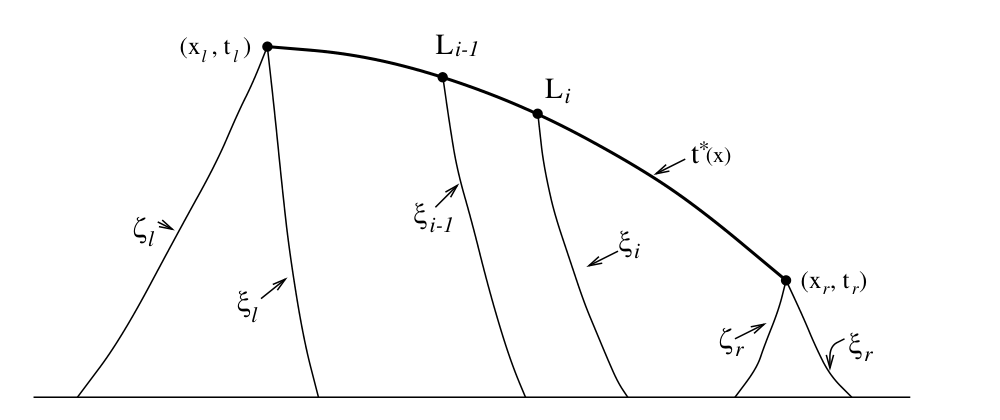
\includegraphics[width=0.85\textwidth]{ch12-fig05-02.png}
\caption{沿类空曲线 $t^*(x)$ 取点列 $L_i$ 并从各点引后向特征线}
\label{figure:ch12-TV特征线}
\end{figure}

\begin{lemma}\label{lemma:ch12-树界}
设 $\mathscr{M}$（或 $\mathscr{N}$）是以 $I_0$ 为根的 1-特征线树（或 2-特征线树）。则
\begin{align}
\mathscr{P}_1(\mathscr{M})+\mathscr{Q}_1(\mathscr{M})&\leqslant c\delta^2(1+V_{\mathscr{M}})\{TV_{[p_-^{I_0}(0),p_+^{I_0}(0)]}z(\cdot,0)+\mathscr{P}_2(\mathscr{F}_{I_0})+\mathscr{Q}_2(\mathscr{F}_{I_0})\},
\label{align:ch12-树界1}\\
\mathscr{P}_2(\mathscr{N})+\mathscr{Q}_2(\mathscr{N})&\leqslant c\delta^2(1+W_{\mathscr{N}})\{TV_{[q_-^{I_0}(0),q_+^{I_0}(0)]}w(\cdot,0)+\mathscr{P}_1(\mathscr{G}_{I_0})+\mathscr{Q}_1(\mathscr{G}_{I_0})\},
\label{align:ch12-树界2}
\end{align}
其中 $V_{\mathscr{M}}$（或 $W_{\mathscr{N}}$）表示
\begin{align}
\sum_{i=0}^{m-1}\{|z_-^{I_iI_{i+1}}-z_S^{I_{i+1}}|+|w_-^{I_iI_{i+1}}-w_S^{I_{i+1}}|\}
\label{align:ch12-V定义}
\end{align}
或
\begin{align}
\sum_{i=0}^{m-1}\{|z_+^{I_iI_{i+1}}-z_S^{I_{i+1}}|+|w_+^{I_iI_{i+1}}-w_S^{I_{i+1}}|\}
\label{align:ch12-W定义}
\end{align}
在 $\mathscr{M}$（或 $\mathscr{N}$）的所有链 $\{I_0,\cdots,I_m\}$ 上的最大值。
\end{lemma}

\begin{proof}
只需验证\eqref{align:ch12-树界1}，另一情形完全类似。由\eqref{align:ch12-P1}与\eqref{align:ch12-Q1}，
\begin{align}
\mathscr{P}_1(\mathscr{M})\leqslant-\sum_{I\in\mathscr{M}}[\Delta w_*^I-\sum_{J\in\mathscr{C}_I}\Delta w_*^J]+\mathscr{Q}_1(\mathscr{M})
=\sum_{\text{极大节点}}\Delta w_*^K-\Delta w_*^{I_0}+\mathscr{Q}_1(\mathscr{M}).
\label{align:ch12-P1 telescoping}
\end{align}
由于 $\Delta w_*^K\leqslant0$，为建立\eqref{align:ch12-树界1}，只需证明
\begin{align}
-\Delta w_*^{I_0}&\leqslant c\delta^2\{TV_{[p_-^{I_0}(0),p_+^{I_0}(0)]}z(\cdot,0)+\mathscr{P}_2(\mathscr{F}_{I_0})+\mathscr{Q}_2(\mathscr{F}_{I_0})\},
\label{align:ch12-根界}\\
\mathscr{Q}_1(\mathscr{M})&\leqslant c\delta^2(1+V_{\mathscr{M}})\{TV_{[p_-^{I_0}(0),p_+^{I_0}(0)]}z(\cdot,0)+\mathscr{P}_2(\mathscr{F}_{I_0})+\mathscr{Q}_2(\mathscr{F}_{I_0})\}.
\label{align:ch12-Q1界}
\end{align}

为证明\eqref{align:ch12-根界}，先用\eqref{align:ch12-出波w}得
\begin{align}
-\Delta w_*^{I_0}=-f(\Delta z^{I_0};z_S^{I_0},w_S^{I_0})\leqslant c\delta^2\Delta z^{I_0},
\label{align:ch12-根界f}
\end{align}
然后为估计 $\Delta z^{I_0}$，将\cref{lemma:ch12-迹差估计}用于 $(\hat x,\hat t)=(\tilde x,\tilde t)=I_0$，$\hat p=p_-^{I_0}$，$\tilde p=p_+^{I_0}$。

现转向\eqref{align:ch12-Q1界}的证明，回忆 $\mathscr{Q}_1(\mathscr{M})$ 的定义\eqref{align:ch12-Q1}。对任意节点 $I\in\mathscr{M}$ 与 $J\in\mathscr{C}_I$，用\eqref{align:ch12-出波w}与\eqref{align:ch12-链节f}得
\begin{align}
\Delta w^{IJ}-\Delta w_*^J&=f(\Delta z^{IJ};z_-^{IJ},w_-^{IJ})-f(\Delta z^{IJ};z_S^J,w_S^J)\nonumber\\
&\quad+f(\Delta z^{IJ};z_S^J,w_S^J)-f(\Delta z^J;z_S^J,w_S^J).
\label{align:ch12-Q1分解}
\end{align}
由函数 $f$ 的性质，
\begin{align}
|f(\Delta z^{IJ};z_-^{IJ},w_-^{IJ})-f(\Delta z^{IJ};z_S^J,w_S^J)|&\leqslant c\delta^2\Delta z^{IJ}\{|z_-^{IJ}-z_S^J|+|w_-^{IJ}-w_S^J|\},
\label{align:ch12-f估计1}\\
|f(\Delta z^{IJ};z_S^J,w_S^J)-f(\Delta z^J;z_S^J,w_S^J)|&\leqslant c\delta^2|\Delta z^{IJ}-\Delta z^J|.
\label{align:ch12-f估计2}
\end{align}
因此，为验证\eqref{align:ch12-Q1界}，须证明
\begin{align}
\sum_{I\in\mathscr{M}}\sum_{J\in\mathscr{C}_I}\Delta z^{IJ}\{|z_-^{IJ}-z_S^J|+|w_-^{IJ}-w_S^J|\}
\leqslant V_{\mathscr{M}}\{\Delta z^{I_0}+\sum_{I\in\mathscr{M}}\sum_{J\in\mathscr{C}_I}|\Delta z^{IJ}-\Delta z^J|\},
\label{align:ch12-Q1归结1}\\
\sum_{I\in\mathscr{M}}\sum_{J\in\mathscr{C}_I}|\Delta z^{IJ}-\Delta z^J|
\leqslant c\{TV_{[p_-^{I_0}(0),p_+^{I_0}(0)]}z(\cdot,0)+\mathscr{P}_2(\mathscr{F}_{I_0})+\mathscr{Q}_2(\mathscr{F}_{I_0})\}.
\label{align:ch12-Q1归结2}
\end{align}

先处理\eqref{align:ch12-Q1归结1}。我们从极大节点出发向根 $\mathscr{M}$ 逐步求和。对 $L\in\mathscr{M}$，令 $\mathscr{M}_L$ 表示以 $L$ 为根且含所有满足 $L<I$ 的 $I\in\mathscr{M}$ 的子树。对某 $K\in\mathscr{M}$，假设
\begin{align}
\sum_{I\in\mathscr{M}_L}\sum_{J\in\mathscr{C}_I}\Delta z^{IJ}\{|z_-^{IJ}-z_S^J|+|w_-^{IJ}-w_S^J|\}\leqslant V_{\mathscr{M}_L}\{\Delta z^L+\sum_{I\in\mathscr{M}_L}\sum_{J\in\mathscr{C}_I}|\Delta z^{IJ}-\Delta z^J|\}
\label{align:ch12-归纳}
\end{align}
对每个 $L\in\mathscr{C}_K$ 成立。因 $\Delta z^L\leqslant\Delta z^{KL}+|\Delta z^{KL}-\Delta z^L|$ 且
\begin{align}
\sum_{L\in\mathscr{C}_K}\Delta z^{KL}\leqslant\Delta z^K,
\label{align:ch12-和KL}
\end{align}
\eqref{align:ch12-归纳}蕴含
\begin{align}
\sum_{I\in\mathscr{M}_K}\sum_{J\in\mathscr{C}_I}\Delta z^{IJ}\{|z_-^{IJ}-z_S^J|+|w_-^{IJ}-w_S^J|\}
&\leqslant\sum_{L\in\mathscr{C}_K}\Delta z^{KL}\{|z_-^{KL}-z_S^L|+|w_-^{KL}-w_S^L|+V_{\mathscr{M}_L}\}\nonumber\\
&\quad+\sum_{L\in\mathscr{C}_K}V_{\mathscr{M}_L}\{|\Delta z^{KL}-\Delta z^L|+\sum_{I\in\mathscr{M}_L}\sum_{J\in\mathscr{C}_I}|\Delta z^{IJ}-\Delta z^J|\}\nonumber\\
&\leqslant V_{\mathscr{M}_K}\{\Delta z^K+\sum_{I\in\mathscr{M}_K}\sum_{J\in\mathscr{C}_I}|\Delta z^{IJ}-\Delta z^J|\}.
\label{align:ch12-归纳步}
\end{align}
于是逐步推导，即得\eqref{align:ch12-Q1归结1}。

还须证明\eqref{align:ch12-Q1归结2}。注意到
\begin{align}
\Delta z^{IJ}-\Delta z^J=[z_+^{IJ}-z_E^J]+[z_S^J-z_-^{IJ}].
\label{align:ch12-差分解}
\end{align}
我们两次应用\cref{lemma:ch12-迹差估计}来估计右端：第一次取 $(\hat x,\hat t)=J$、$(\tilde x,\tilde t)=I$、$\hat p=p_+^J$、$\tilde p=p_+^{IJ}$；第二次取 $(\hat x,\hat t)=I$、$(\tilde x,\tilde t)=J$、$\hat p=p_-^{IJ}$、$\tilde p=p_-^J$。在两种情形，连接 $I$ 到 $J$ 的特征线 $\chi_-^J$ 的弧都充当 $\bar t$。我们合并两种情形下\eqref{align:ch12-迹差1}的推导：从 $p_+^J$ 图像上任一点 $K$ 发出的特征线 $\phi_-^K$ 总被 $p_+^{IJ}$ 的图像截取，从不被 $\chi_-^J$ 的图像截取；另一方面，从 $p_-^{IJ}$ 图像上点 $K$ 发出并穿过 $\chi_-^J$ 图像的 $\phi_-^K$ 可延长直至与 $p_+^J$ 的图像相交。因此公共 $\bar t$ 的贡献抵消，剩下估计
\begin{align}
|\Delta z^{IJ}-\Delta z^J|\leqslant TV_{[p_-^{IJ}(0),p_-^J(0)]}z(\cdot,0)+TV_{[p_+^J(0),p_+^{IJ}(0)]}z(\cdot,0)+\mathscr{P}_2(\mathscr{F}_{IJ})+\mathscr{Q}_2(\mathscr{F}_{IJ}),
\label{align:ch12-差界}
\end{align}
其中 $\mathscr{F}_{IJ}$ 定义为
\begin{align}
\mathscr{F}_{IJ}=\{(x,t):0\leqslant t<t_I,\ p_-^{IJ}(t)\leqslant x\leqslant p_+^{IJ}(t)\}\cap\overline{\mathscr{F}_J^C}.
\label{align:ch12-FIJ}
\end{align}

当 $(I,J)$ 与 $(K,L)$ 是任意两条不同链节（允许 $I=K$）时，区间 $(p_-^{IJ}(0),p_-^J(0))$、$(p_+^J(0),p_+^{IJ}(0))$、$(p_-^{KL}(0),p_-^L(0))$ 与 $(p_+^L(0),p_+^{KL}(0))$ 两两不交；同样，集合 $\mathscr{F}_{IJ}$ 与 $\mathscr{F}_{KL}$ 的内部不交。因此，由\cref{lemma:ch12-不相交求和}，先对 $J\in\mathscr{C}_I$ 再对 $I\in\mathscr{M}$ 总计\eqref{align:ch12-差界}，即得\eqref{align:ch12-Q1归结2}。证明完成。
\end{proof}

\begin{lemma}\label{lemma:ch12-相互作用有界}
在\cref{theorem:ch12-TV界}的假设下，若 $\mathscr{H}$ 表示由 $\zeta_\ell$、$\xi_r$、$t^*$ 与 $x$ 轴的图像所围成的区域，则
\begin{align}
\mathscr{P}_1(\mathscr{H})+\mathscr{Q}_1(\mathscr{H})+\mathscr{P}_2(\mathscr{H})+\mathscr{Q}_2(\mathscr{H})
\leqslant c\delta^2\{TV_{[\zeta_\ell(0),\xi_r(0)]}z(\cdot,0)+TV_{[\zeta_\ell(0),\xi_r(0)]}w(\cdot,0)\}.
\label{align:ch12-相互作用有界}
\end{align}
\end{lemma}

\begin{proof}
考虑含于 $\mathscr{H}$ 的任一不交 1-特征线树族 $\mathscr{J}$。若 $I$ 与 $J$ 是 $\mathscr{J}$ 中任意两棵树的根，则 $(p_-^I(0),p_+^I(0))$ 与 $(p_-^J(0),p_+^J(0))$ 是含于 $(\zeta_\ell(0),\xi_r(0))$ 的不交区间；且 $\mathscr{F}_I$ 与 $\mathscr{F}_J$ 是 $\mathscr{H}$ 的内部不交子集。因此，结合\cref{lemma:ch12-不相交求和}与\cref{lemma:ch12-树界}，推得
\begin{align}
\mathscr{P}_1(\mathscr{H})+\mathscr{Q}_1(\mathscr{H})\leqslant c\delta^2(1+V_{\mathscr{H}})\{TV_{[\zeta_\ell(0),\xi_r(0)]}z(\cdot,0)+\mathscr{P}_2(\mathscr{H})+\mathscr{Q}_2(\mathscr{H})\},
\label{align:ch12-P1Q1H}
\end{align}
其中 $V_{\mathscr{H}}$ 表示图像含于 $\mathscr{H}$ 的所有 1-特征线上 $(z,w)$ 迹的总变差上确界。类似地，
\begin{align}
\mathscr{P}_2(\mathscr{H})+\mathscr{Q}_2(\mathscr{H})\leqslant c\delta^2(1+W_{\mathscr{H}})\{TV_{[\zeta_\ell(0),\xi_r(0)]}w(\cdot,0)+\mathscr{P}_1(\mathscr{H})+\mathscr{Q}_1(\mathscr{H})\},
\label{align:ch12-P2Q2H}
\end{align}
其中 $W_{\mathscr{H}}$ 表示图像含于 $\mathscr{H}$ 的所有 1-特征线上 $(z,w)$ 迹的总变差上确界。

\eqref{align:ch12-TV传递1}与\eqref{align:ch12-TV传递2}中的常数不依赖于特定的 $t^*$，只要 $\mathscr{H}$ 保持固定。特别地，我们可取含于 $\mathscr{H}$ 的任一 1-特征线或 2-特征线作为 $t^*$ 来应用这些估计。因此，
\begin{align}
(1-c\delta^2)V_{\mathscr{H}}&\leqslant TV_{[\zeta_\ell(0),\xi_r(0)]}z(\cdot,0)+TV_{[\zeta_\ell(0),\xi_r(0)]}w(\cdot,0)\nonumber\\
&\quad+2\{\mathscr{P}_1(\mathscr{H})+\mathscr{Q}_1(\mathscr{H})+\mathscr{P}_2(\mathscr{H})+\mathscr{Q}_2(\mathscr{H})\},
\label{align:ch12-VH}\\
(1-c\delta^2)W_{\mathscr{H}}&\leqslant TV_{[\zeta_\ell(0),\xi_r(0)]}z(\cdot,0)+TV_{[\zeta_\ell(0),\xi_r(0)]}w(\cdot,0)\nonumber\\
&\quad+2\{\mathscr{P}_1(\mathscr{H})+\mathscr{Q}_1(\mathscr{H})+\mathscr{P}_2(\mathscr{H})+\mathscr{Q}_2(\mathscr{H})\}.
\label{align:ch12-WH}
\end{align}
结合\eqref{align:ch12-P1Q1H}、\eqref{align:ch12-P2Q2H}、\eqref{align:ch12-VH}、\eqref{align:ch12-WH}并回忆\eqref{align:ch12-初值总变差}，当 $\delta$ 充分小时即推得\eqref{align:ch12-相互作用有界}。证明完成。
\end{proof}

现结合\cref{lemma:ch12-TV传递}与\cref{lemma:ch12-相互作用有界}。由于 $\mathscr{F}$ 与 $\mathscr{G}$ 是 $\mathscr{H}$ 的子集，\eqref{align:ch12-TV传递1}、\eqref{align:ch12-TV传递2}与\eqref{align:ch12-相互作用有界}共同蕴含\eqref{align:ch12-TV界z}与\eqref{align:ch12-TV界w}。这样\cref{theorem:ch12-TV界}的断言即已建立。

除充当\cref{theorem:ch12-TV界}证明中的垫脚石外，\cref{lemma:ch12-相互作用有界}还揭示：第一与第二特征族波的自相互作用总量（分别由 $\mathscr{P}_1$、$\mathscr{P}_2$ 度量），以及异族波相互作用总量（由 $\mathscr{Q}_1$、$\mathscr{Q}_2$ 度量），均有界并由初始数据的总变差控制。

在我们推导\eqref{align:ch12-TV界z}时，初始数据被视为多值的，其总变差按允许取值中"最不利"的选取来评估。按此约定，$z(x,0)$ 的取值集要么被限制在 $z(x-,0)$ 与 $z(x+,0)$ 之间，要么距 $z(x+,0)$ 在 $c|w(x+,0)-w(x-,0)|^3$ 范围内；$w(x,0)$ 有类似性质。因此，当 $(z(\cdot,0),w(\cdot,0))$ 被重新归一化为单值时（例如在 $\xi_\ell(0)$ 与 $\zeta_r(0)$ 处从右连续、在其他点从左连续），\eqref{align:ch12-TV界z}仍以调整后的常数 $c$ 成立。

\end{document}
